\documentclass{beamer}
\usepackage{hyperref} %links and URLS
\usepackage{graphicx} % Required for inserting images
\usepackage[linguistics]{forest} %calls tikz, draws trees
\usepackage{multicol} %adds columns
\usepackage{gb4e} %for formatting examples, works with leipzig and multicol
\primebars %setting for gb4e, adds bars for X-bar notation, allows switch between bar or %'%
\noautomath
\usepackage{tipa} % IK
\usepackage[T1]{fontenc} %Make sure to be able to get accented characters etc
\usepackage[utf8]{inputenc}
\usepackage[normalem]{ulem} %adds strikethrough and other commands
\usepackage{setspace}
\usepackage{pifont} %allows dingbats to be called (for the "crosses" and "ticks" defined below)

\title{LEL2A: Syntax}
%\author{Instructor: Itamar Kastner}
\date{Semester 1, 2025--26}%changed to current academic year


\setbeamertemplate{footline}[frame number]
\setbeamertemplate{blocks}[rounded][shadow=true]
\setbeamertemplate{navigation symbols}{}
\usecolortheme[RGB={0,51,102}]{structure}
\setbeamercolor{alerted text}{fg=red}

\newcommand{\cmark}{\ding{51}}
\newcommand{\xmark}{\ding{55}}
\newcommand\trace{\rule[-0.5ex]{0.5cm}{.4pt}}

\subtitle{Topic 12: \emph{wh}-questions}

\begin{document}
\maketitle

\frame{\frametitle{Recap}
    \begin{block}{Topic 11 skills}
    \begin{itemize}
        \item[11a]{Account for the behaviour of passive movement, including any relevant restrictions, within the framework developed.}
        \item[11b]{\sout{Identify relevant locality constraints on A-movement.}}
    \end{itemize}
    \end{block}
}

\frame{\frametitle{Topic 12}
 \begin{block}{Topic 12 skills}
    \begin{itemize}
        \item[12a]{Implement a movement-based analysis of \emph{wh}-movement.}
        \item[12b]{\sout{Account for differences in the order of subjects and auxiliary verbs in question formation.}}
    \end{itemize}
    \end{block}
}


\frame{
    What are two different kinds of answers to this question:

    \bigskip
    \ea When did she say they would launch her perfume?
    \z

}

\frame{
    \ea What do they admire?
    \z
}


\frame{  \centering \small
    \hspace{-5em}
    \begin{forest}
    [CP
        [DP [what, roof, name=matrixCP]]
        [C'
            [C [do, name=matrixC]]
            [IP
                [DP [they, roof, name=matrixIP]]
                [I'
                    [I [\sout{do}, name=matrixI]]
                    [VP
                        [DP [\sout{they}, roof, name=matrixVP]]
                        [V'
                            [V\\admire]
                            [DP [\sout{what}, roof, name=whtrace]]
                        ]
                    ]
                ]
            ]
        ]
    ]
    \draw[->,dotted] (whtrace) to[out=south west,in=south west] (matrixCP);
    \draw[->,dotted] (matrixVP) to[out=south west,in=south west] (matrixIP);
    \draw[->,dotted] (matrixI) to[out=south west,in=south west] (matrixC);
    \end{forest}
}

\frame{
    \ea Who saw a ghost?
    \z
}

\frame{ \centering
    \begin{forest}
    [CP
        [DP [who, roof, name=specCP]]
        [C'
            [C ]
            [IP
                [DP [\sout{who}, roof, name=specIP]]
                [I'
                    [I ]
                    [VP
                        [DP [\sout{who}, roof, name=specVP]]
                        [V'
                            [V\\saw]
                            [DP [a ghost, roof]]
                        ]
                    ]
                ]
            ]
        ]
    ]
    \draw[->,dotted] (specVP) to[out=south west,in=south] (specIP);
    \draw[->,dotted] (specIP) to[out=south west,in=south west] (specCP);
    \end{forest}
}

\frame{
    \ea Who seems to see ghosts?
    \z
}

\frame{ \centering \tiny
    \begin{forest}
    [CP
        [DP [who, roof, name=matrixCP]]
        [C'
            [C ]
            [IP
                [DP [who, roof, name=matrixIP]]
                [I'
                    [I ]
                    [VP
                        [\phantom{X} ]
                        [V'
                            [V\\seems]
                            [CP
                                [DP [who, roof, name=specCP]]
                                [C'
                                    [C ]
                                    [IP
                                        [DP [\sout{who}, roof, name=specIP]]
                                        [I'
                                            [I\\to]
                                            [VP
                                                [DP [\sout{who}, roof, name=specVP]]
                                                [V'
                                                    [V\\see]
                                                    [DP [ghosts, roof]]
                                                ]
                                            ]
                                        ]
                                    ]
                                ]
                            ]                        
                        ]
                    ]
                ]
            ]
        ]
    ]
    \draw[->,dotted] (specVP) to[out=south west,in=south] (specIP);
    \draw[->,dotted] (specIP) to[out=south west,in=south] (specCP);
    \draw[->,dotted] (specCP) to[out=south west,in=south] (matrixIP);
    \draw[->,dotted] (matrixIP) to[out=south west,in=south west] (matrixCP);
    \end{forest}
}

\frame{
    \ea When did she say they would launch her perfume?
    \z
}

\frame{ \tiny
    \hspace*{-3em}
    \begin{forest}
    [CP
        [AdvP [when, roof, name=matrixCP]]
        [C'
            [C [did, name=matrixC]]
            [IP
                [DP [she, roof, name=matrixIP]]
                [I'
                    [I [\sout{did}, name=matrixI]]
                    [VP
                        [DP [\sout{she}, roof, name=matrixVP]]
                        [V'
                            [V\\say]
                            % [(CP)
                                % [(\sout{when}), name=whmid ]
                                % [(C')
                                    % [(C) ]
                                    [IP 
                                        [DP [they, roof, name=lowIP]]
                                        [I'
                                            [I\\would]
                                            [VP
                                                [DP [\sout{they}, roof, name=lowVP]]
                                                [V'
                                                    [V' [launch her perfume, 
                                            roof]]
                                                    [AdvP [when, roof, name=whtrace]]       
                                                ]
                                            ]
                                        ]
                                    ]
                                % ]
                            % ]
                        ]
                    ]
                ]
            ]
        ]
    ]
    % \draw[->,dashed] (whtrace) to[out=south west,in=south] (whmid);
    % \draw[->,dashed] (whmid) to[out=south west,in=south west] (matrixCP);
    \draw[->,dotted] (whtrace) to[out=south west,in=south west] (matrixCP);
    \draw[->,dotted] (matrixVP) to[out=south west,in=south west] (matrixIP);
    \draw[->,dotted] (lowVP) to[out=south west,in=south west] (lowIP);
    \draw[->,dotted] (matrixI) to[out=south west,in=south west] (matrixC);
    \end{forest}
}

\frame{ \tiny
    \hspace*{-3em}
    \begin{forest}
    [CP
        [AdvP [when, roof, name=matrixCP]]
        [C'
            [C [did, name=matrixC]]
            [IP
                [DP [she, roof, name=matrixIP]]
                [I'
                    [I [\sout{did}, name=matrixI]]
                    [VP
                        [DP [\sout{she}, roof, name=matrixVP]]
                        [V'
                            [V\\say]
                            [(CP)
                                [(\sout{when}), name=whmid ]
                                [(C')
                                    [(C) ]
                                    [IP 
                                        [DP [they, roof, name=lowIP]]
                                        [I'
                                            [I\\would]
                                            [VP
                                                [DP [\sout{they}, roof, name=lowVP]]
                                                [V'
                                                    [V' [launch her perfume, 
                                            roof]]
                                                    [AdvP [when, roof, name=whtrace]]       
                                                ]
                                            ]
                                        ]
                                    ]
                                ]
                            ]
                        ]
                    ]
                ]
            ]
        ]
    ]
    \draw[->,dashed] (whtrace) to[out=south west,in=south] (whmid);
    \draw[->,dashed] (whmid) to[out=south west,in=south west] (matrixCP);
    \draw[->,dotted] (whtrace) to[out=south west,in=south west] (matrixCP);
    \draw[->,dotted] (matrixVP) to[out=south west,in=south west] (matrixIP);
    \draw[->,dotted] (lowVP) to[out=south west,in=south west] (lowIP);
    \draw[->,dotted] (matrixI) to[out=south west,in=south west] (matrixC);
    \end{forest}
}
\frame{ \small
    \begin{forest}
    [CP
        [AdvP [when, roof, name=matrixCP]]
        [C'
            [C [did, name=matrixC]]
            [IP
                [DP [she, roof, name=matrixIP]]
                [I'
                    [I [\sout{did}, name=matrixI]]
                    [VP
                        [DP [\sout{she}, roof, name=matrixVP]]
                        [V'
                            [V'
                                [V\\say]
                                [IP [they would launch her perfume, roof]]
                            ]
                            [AdvP [when, roof, name=whtrace]]
                        ]
                    ]
                ]
            ]
        ]
    ]
    \draw[->,dotted] (whtrace) to[out=south west,in=south west] (matrixCP);
    \draw[->,dotted] (matrixVP) to[out=south west,in=south west] (matrixIP);
    \draw[->,dotted] (matrixI) to[out=south west,in=south west] (matrixC);
    \end{forest}
}


\frame{\frametitle{Summary}
  \begin{block}{Topic 12 skills}
    \begin{itemize}
        \item[12a]{Implement a movement-based analysis of \emph{wh}-movement.}
        \item[12b]{\sout{Account for differences in the order of subjects and auxiliary verbs in question formation.}}
    \end{itemize}
    \end{block}

    We also discussed:
    \begin{itemize}
        \item I-to-C movement.
    \end{itemize}

    Research Skills:
    \begin{itemize} \small
    \item[M1]{State a hypothesis clearly}
    \item[M2]{Present data in support of a hypothesis}
    \item[M3]{Define the conditions under which a hypothesis would be refuted}
    \item[M4]{Present data to refute a hypothesis}
    \item[M5]{Consider the limitations of a diagnostic test when interpreting the results}
    \end{itemize}
}

\frame{\frametitle{The puzzles}
    \begin{itemize}
        \item Puzzle 1
        \item Puzzle 2
        \item Puzzle 3
    \end{itemize}
}

\frame{\frametitle{LEL2A syntax}
    Syntax is about:
        \begin{enumerate}
            \item Looking for generalizations.
            \item Building a formal theory.
            \item Establishing some assumptions (e.g.~``Always have a bar-level'').
            \item Establish tests (``is this an argument or a modifier?'').
            \item Use the assumptions to derive the generalizations (e.g.~one structural difference between control and raising predicts a number of empirical differences).
        \end{enumerate}
        
            \begin{columns}
                \begin{column}{0.8\textwidth}
                    (Somehow combining all these different skills and types of knowledge within a month or two) 
                \end{column}
                \begin{column}{0.2\textwidth}
                    
\includegraphics[width=0.99\linewidth]{Images/slayed.png}
                \end{column}
            \end{columns}
        
}

\frame{\frametitle{What I learned}
    \begin{enumerate}
        \item Requiring some work in advance, but also going through it together in class (``teaching'').
        \item Drawing trees together, and giving clean final versions for reference.
        \item Varying in-class activities.
        \item Multiple opportunities to demonstrate a skill.
    \end{enumerate}

    \ding{228} I'll return to ask for your reflections at the end of the year!
}

\frame{\frametitle{What I learned} \centering
    Students understand the assignment.
    
    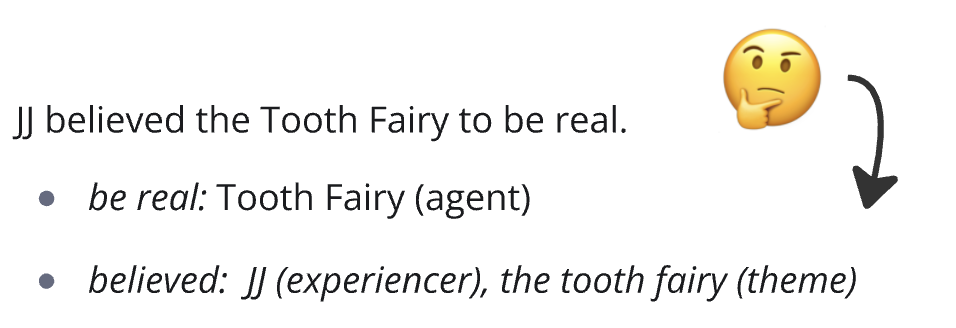
\includegraphics[width=0.35\linewidth]{Images/toothfairy.png}
    
    
\includegraphics[width=0.45\linewidth]{Images/objection.jpeg}
    
    
\includegraphics[width=0.6\linewidth]{Images/spnuun.png}
}


\end{document}
